% ==========================================================
% Template for Internship / Term Project Report
% Duration: 3 months | Length: 4 pages + References
% ==========================================================

\documentclass[twocolumn]{article}
\usepackage{spconf,amsmath,graphicx,hyperref}

% -------------------------
% Additional useful packages
% -------------------------
\usepackage{booktabs}
\usepackage{enumitem}
\usepackage{stfloats}
\usepackage{microtype}
\usepackage{xcolor}

\graphicspath{{reports/figures/}}

% -------------------------
% Title and Author Info
% -------------------------
\title{Monsoon Sentinel (Part 1): Embedded Sensor Interfacing, Resilient Telemetry, and Physical Dataset Acquisition Testbed}

\name{Ganesha N Sai \textit{(Roll Number: 23035010072)}}

\address{
Term Project Report\\
Trimester  8 \\[0.5em]
\textit{B.Sc. (Honours) Data Science and Artificial Intelligence}\\
\textit{Indian Institute of Technology Guwahati, India}\\
\texttt{ganesha.sai@op.iitg.ac.in}
}

\begin{document}
\ninept
\maketitle

% ==========================================================
% Abstract
% ==========================================================
\begin{abstract}
Before deploying edge machine learning models on embedded systems microcontrollers that cannot hold large amounts of data, acquiring clean, deterministic, and uncorrupted sensor datasets is essential. This report presents Part 1 of the Monsoon Sentinel project: the embedded hardware prototyping, driver implementation, and serial data collection pipeline designed to capture physical motion regimes. Using an STM32 Nucleo-F401RE microcontroller (ARM Cortex-M4F) and an MPU-6050 6-Degrees of Freedom IMU over standard-mode $I^2\text{C}$ (100~kHz), I implement a 100~Hz ($T_s = 10.0$~ms) sampling loop streaming across a 115,200~baud UART link. I perform a execution budget audit, proving that synchronous polling I/O stalls the CPU for 49.8\% of each epoch. I resolve critical embedded failure modes including $I^2\text{C}$ slave bus lockups and operating system serial buffer overruns. Using an elastic ruler cantilever and controlled wind sources, I generate five distinct motion regimes. The data acquisition pipeline is verified across a 12-test automated unit test suite checking sampling rates, clock jitter, dynamic range saturation, and energy conservation. In total, 12,348 continuous windows (7,922.45~seconds) were logged across 22 clean datasets, establishing the benchmark for an embedded systems classifier.
\end{abstract}

% ==========================================================
% Keywords
% ==========================================================
\begin{keywords}
Embedded Systems, Sensor Interfacing, STM32F401RE, $I^2\text{C}$, Serial Telemetry, Test Suite.
\end{keywords}

% ==========================================================
\section{Introduction}
% ==========================================================
Real-time monitoring of moving mechanical structures such as marine buoys, towers, and elevated infrastructure under severe wind gusts requires reliable, edge-deployed sensing units. The overarching goal of the Monsoon Sentinel project is to develop an edge-computing smart sensing node capable of recognizing various disturbance regimes directly on-device and classifying them using quantized models.

However, machine learning models running on microcontrollers are fundamentally constrained by the quality of their training datasets. In feature engineering and signal processing, calculations such as the Fast Fourier Transform (FFT) require strict continuity in time. If in the acquisition of a dataset, frame drops, timing jitters, or hung data reading occurs due to peripheral bus collisions or other reasons, downstream machine learning models fail due to bad data.

This project constitutes \textbf{Part 1 (Data Collection \& Telemetry Pipeline)} of a two-term submission. It addresses the embedded systems, sensor interfacing, hardware instrumentation, and dataset curation required to establish an uncorrupted physical foundational dataset setup.

% ==========================================================
\section{Problem Statement and Objectives}
% ==========================================================

\subsection{Problem Statement}
Acquiring physical kinetic vibration datasets on microcontrollers is difficult due to hardware reliability constraints. At 100~Hz sampling rates, synchronous bus transactions take up most of the core compute cycle time, loose breadboard wiring causes catastrophic $I^2\text{C}$ slave line-clamping hangs, and operating system disk latencies induce silent serial buffer drops. Rather than training models on synthetic or unverified internet data, an end-to-end, resilient acquisition pipeline must be physically made, benchmarked, and mathematically verified.

\subsection{Objectives}
The primary objectives executed during this project were:
\begin{enumerate}[noitemsep]
    \item To design and wire a 6-DOF IMU sensing rig using the STM32F401RE microcontroller with dedicated logic analyzer instrumentation tap points.
    \item To implement a deterministic 100~Hz sampling firmware loop and quantify core cycle utilization via a cycle-accurate latency budget.
    \item To engineer an algorithmic 9-clock bus-clear sequence resolving permanent $I^2\text{C}$ slave line-clamping lockups.
    \item To develop a multi-threaded serial logging engine with non-fatal stale-data checkpoints to eliminate packet loss.
    \item To construct an automated 12-test validation test suite asserting temporal cadence, noise floor bounds, and Parseval spectral energy conservation.
    \item To physically record and curate a 5-regime motion dataset spanning over 12,000 feature windows.
\end{enumerate}

% ==========================================================
\section{Methodology / Approach}
% ==========================================================

\subsection{Overall Workflow}
The end-to-end acquisition and validation pipeline flows from physical mechanical excitation to automated feature verification, as illustrated in Fig.~\ref{fig:workflow_block}.

\begin{figure}[htbp]
    \centering
    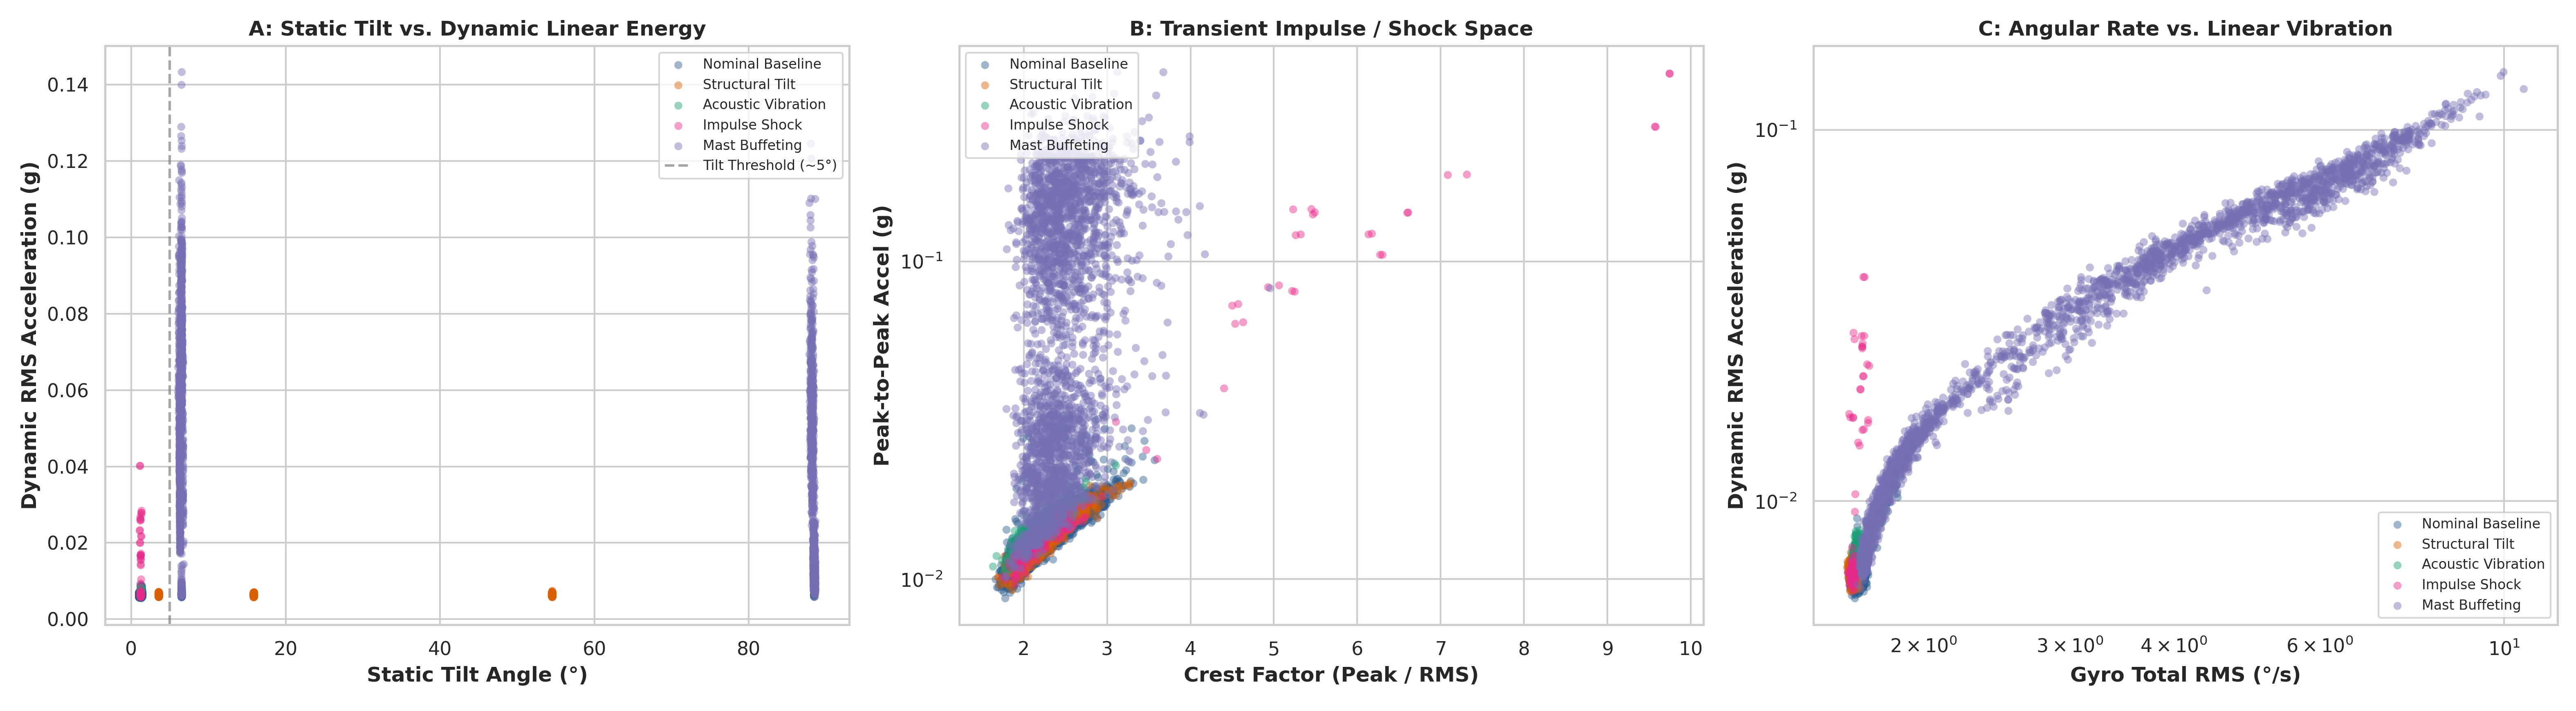
\includegraphics[width=\columnwidth]{reports/figures/eda_scatter_separability.png}
    \caption{Three-panel 2D scatter plots of the recorded dataset. Panel A isolates static tilt from dynamic energy. Panel B highlights impulse shocks via Crest Factor and Peak-to-Peak acceleration. Panel C shows the clean correlation between linear vibration and rotational motion during wind excitation.}
    \label{fig:workflow_block}
\end{figure}

\subsection{Hardware Architecture and Testbed Setup}
The compute engine is an STM32 Nucleo-F401RE board featuring an ARM Cortex-M4F core operating at $f_{\text{SYSCLK}} = 84.0$~MHz. The clock tree uses the internal 16~MHz HSI oscillator coupled to the main PLL ($M=16, N=336, P=4, Q=7$). The AHB and APB2 buses run at 84~MHz, while the APB1 peripheral bus is prescaled to 42~MHz with 2 Flash wait states.

Motion sensing uses an InvenSense MPU-6050 6-DOF IMU configured for $\pm 2g$ ($16,384~\text{LSB}/g$) and $\pm 250^\circ/\text{s}$ ($131.0~\text{LSB}/(^\circ/\text{s})$). The sensor is interfaced via $I^2\text{C}1$ on pins PB8 (SCL) and PB9 (SDA) with $4.7~\text{k}\Omega$ pull-up resistors to 3.3~V, operating in Standard Mode (100.0~kHz). Telemetry streams over USART2 (TX on PA2, RX on PA3) at 115,200~baud (8N1). To verify protocol timing, a Muse Lab nanoDLA 24~MHz logic analyzer was connected to PB8, PB9, and PA2.

To generate motion patterns, an elastic cantilever ruler rig (30~cm length) was clamped rigidly at the base with the MPU-6050 mounted at the tip. Variable-speed blowers provided face-on wind excitation, calibrated wedges established static tilts ($0^\circ$ to $55^\circ$), and physical taps generated impulse shocks.

\begin{figure}[htbp]
    \centering
    \begin{minipage}{0.48\columnwidth}
        \centering
        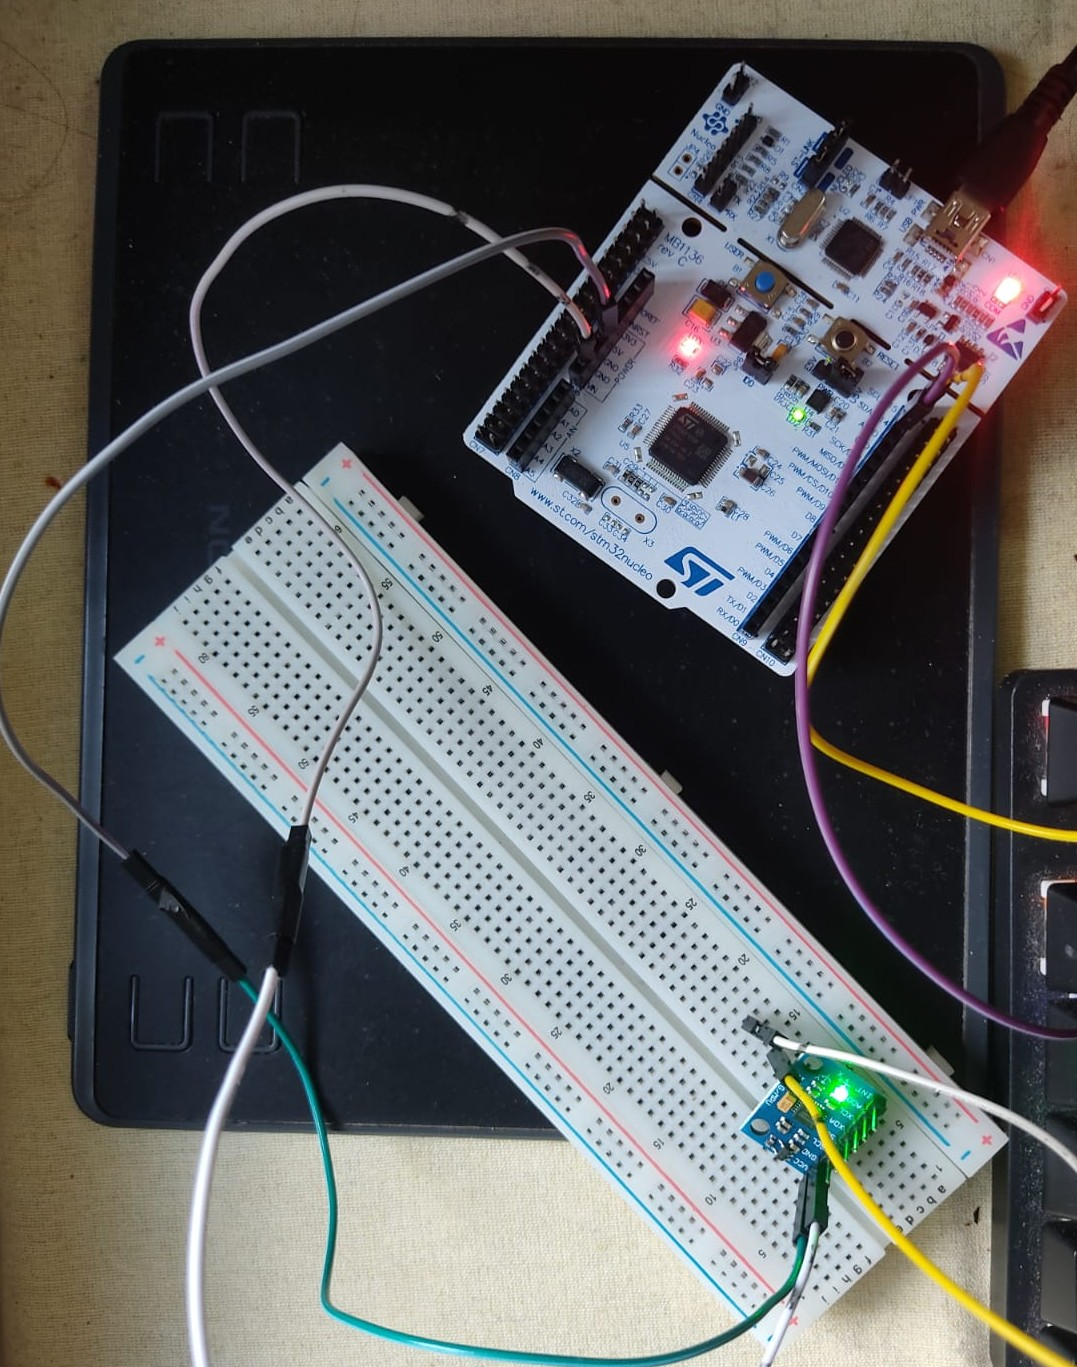
\includegraphics[width=\textwidth]{tabletop.jpeg}
        \caption{Tabletop bench setup.}
        \label{fig:tabletop}
    \end{minipage}\hfill
    \begin{minipage}{0.48\columnwidth}
        \centering
        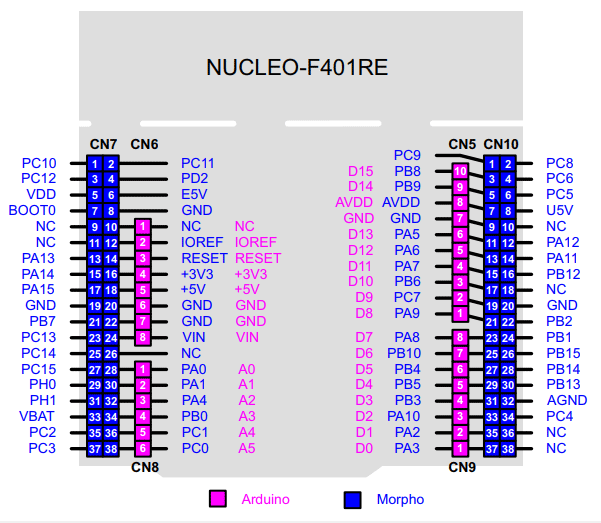
\includegraphics[width=\textwidth]{stm32_pinout.png}
        \caption{STM32 to IMU pinout.}
        \label{fig:pinout}
    \end{minipage}
    \vspace{0.5em}
    \begin{minipage}{0.48\columnwidth}
        \centering
        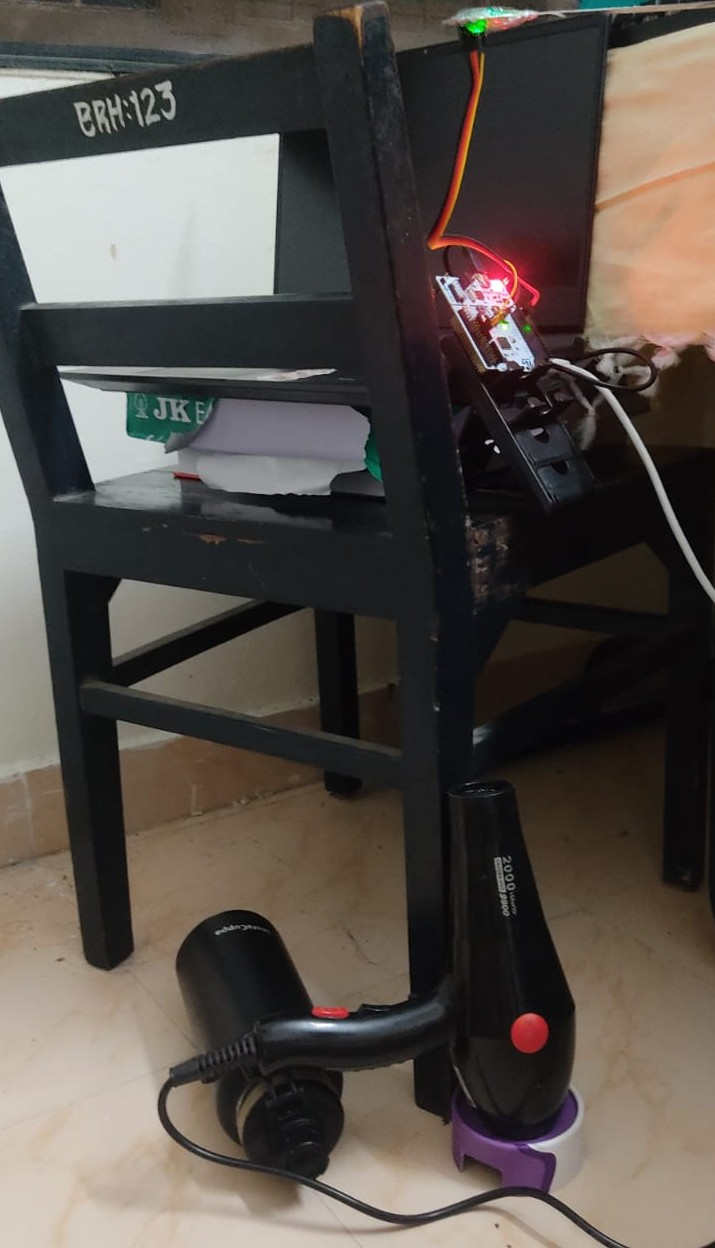
\includegraphics[width=\textwidth]{fan_ruler.jpeg}
        \caption{Cantilever ruler rig.}
        \label{fig:fan_ruler}
    \end{minipage}\hfill
    \begin{minipage}{0.48\columnwidth}
        \centering
        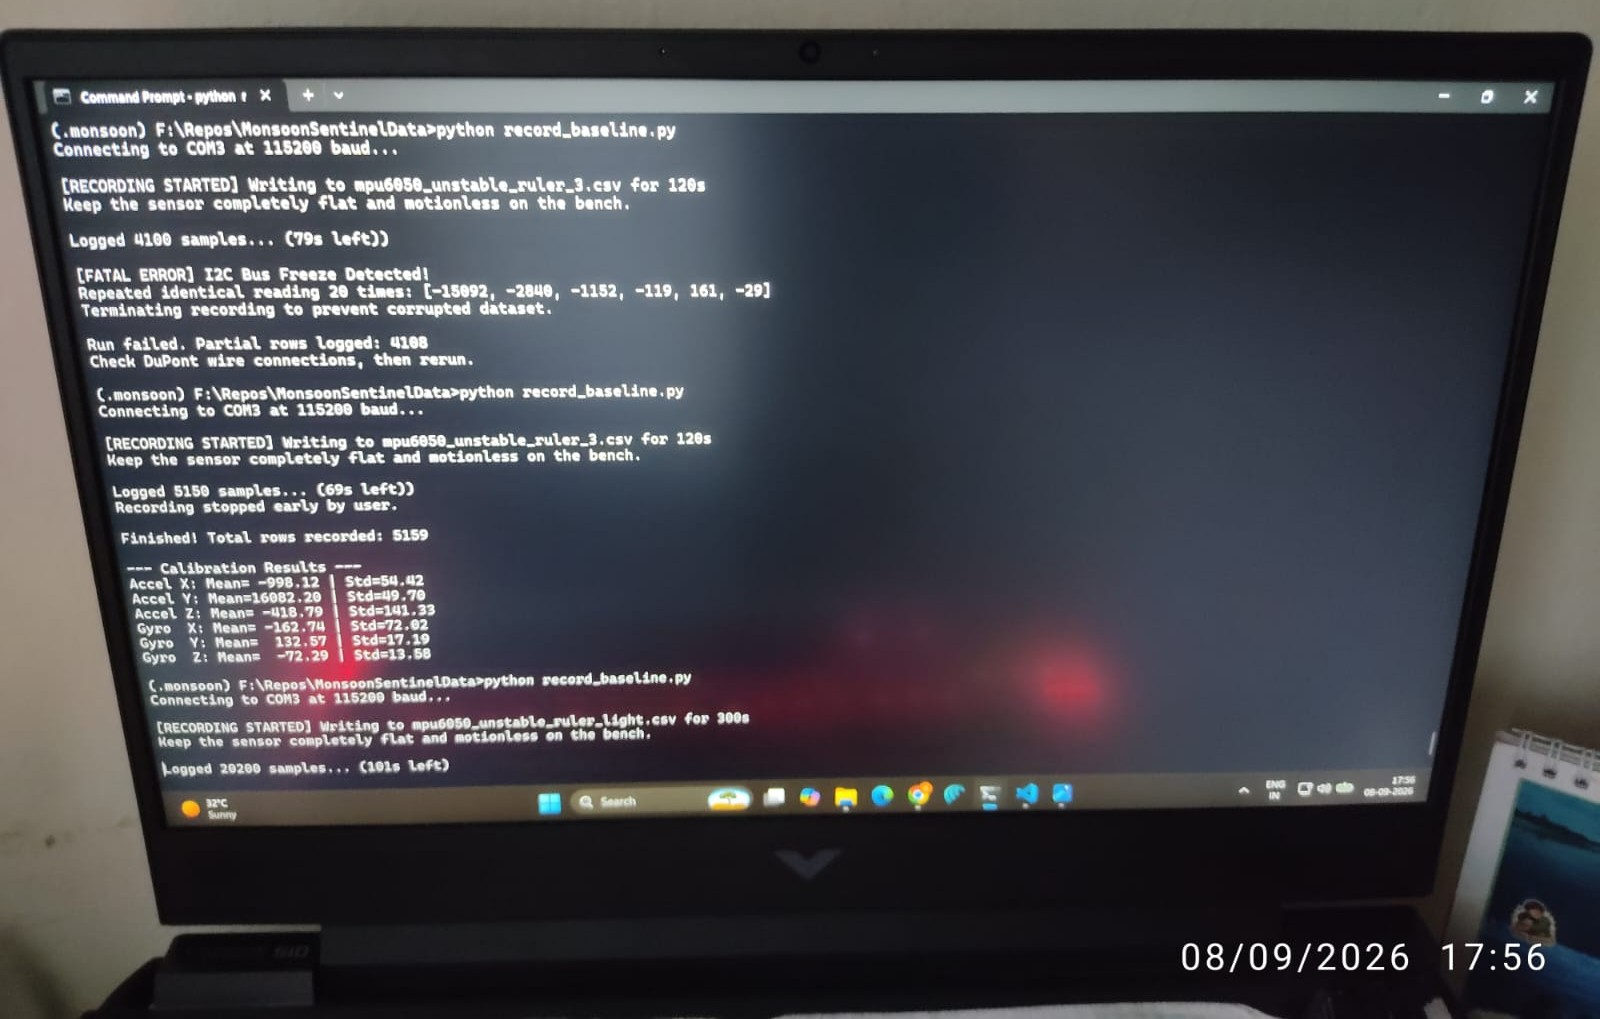
\includegraphics[width=\textwidth]{screen_data.jpeg}
        \caption{Live telemetry stream.}
        \label{fig:screen_data}
    \end{minipage}
\end{figure}

\subsection{Firmware Sampling and Timing Budget}
The firmware runs in an explicit polling loop within \texttt{main.c}. Every 10.0~ms ($100~\text{Hz}$), evaluated via \texttt{HAL\_GetTick()}, the MCU executes a 14-byte burst read starting at register \texttt{0x3B} (\texttt{ACCEL\_XOUT\_H}), capturing 6 bytes of acceleration, 2 bytes of temperature, and 6 bytes of gyro rates. The raw int16 values are formatted via \texttt{sprintf} and transmitted over UART.

Table~\ref{tab:timing_budget} details the cycle-accurate execution profile measured across the 84~MHz platform. Synchronous I/O consumes 4.980~ms out of every 10.0~ms cycle ($49.80\%$ core wait-state load), leaving 5.020~ms ($50.20\%$) idle margin.

% Auto-generated by generate_report_tables.py
\begin{table}[htbp]
\centering
\caption{STM32F401RE Hardware Execution \& Bus Blocking Budget ($f_{\text{CPU}} = 84\,\text{MHz}$, $T_s = 10.0\,\text{ms}$, 100\,Hz Cadence)}
\label{tab:timing_budget}
\begin{tabular}{llcccc}
\toprule
\textbf{Pipeline Operation} & \textbf{Peripheral Mode} & \textbf{Bus Clock} & \textbf{Duration (ms)} & \textbf{CPU Cycles} & \textbf{Core Load (\%)} \\
\midrule
I2C Sensor Burst Read (14\,B) & Synchronous Polling & 100\,kHz (Std)  & 1.500 & 126,000 & 15.00\% \\
ASCII String Formatting       & In-Memory (`sprintf`) & 84\,MHz (Core)  & 0.008 & 672     & 0.08\% \\
UART Telemetry TX (~40\,B)    & Synchronous Polling & 115.2\,kbaud    & 3.472 & 291,648 & 34.72\% \\
\midrule
\textbf{Total Blocking Overhead} & \textbf{Synchronous Wait} & \textbf{--} & \textbf{4.980} & \textbf{418,320} & \textbf{49.80\%} \\
SysTick Polling Idle Budget    & Main Loop Busy-Wait & 84\,MHz (Core)  & 5.020 & 421,680 & 50.20\% \\
\midrule
\textbf{Total Available Budget} & \textbf{100\,Hz Loop Period} & \textbf{84\,MHz} & \textbf{10.000} & \textbf{840,000} & \textbf{100.00\%} \\
\bottomrule
\end{tabular}
\end{table}


\subsection{Bus Fault Recovery and Data Reading}
When mechanical vibration induces clock glitches, the MPU-6050 can latch SDA low during a read transaction. Because SDA cannot rise, the hardware master detects a permanent bus collision, causing \texttt{HAL\_I2C\_Mem\_Read} to time out continuously (100~ms timeout) and collapsing throughput to $<10$~Hz.

I resolve this by embedding a 9-clock manual recovery routine prior to peripheral configuration:
\begin{enumerate}[noitemsep]
    \item Disable the $I^2\text{C}$ clock (\texttt{\_\_HAL\_RCC\_I2C1\_CLK\_DISABLE}).
    \item Reconfigure PB8 and PB9 as standard GPIO Open-Drain outputs.
    \item Clock SCL manually for 9 cycles at 100~kHz, forcing the slave to advance its internal shift register and release SDA.
    \item Assert a manual STOP condition (SCL high, SDA low $\to$ high).
    \item Re-initialize $I^2\text{C}1$ via \texttt{HAL\_I2C\_Init}.
\end{enumerate}

Reading data onto the PC uses a multi-threaded Python engine (\texttt{record\_telemetry.py}). A dedicated thread reads non-blocking serial frames into an in-memory queue (\texttt{queue.Queue(maxsize=10000)}), decoupling transport from CSV disk writes and eliminating serial buffer drops.

% ==========================================================
\section{Experiments and Results}
% ==========================================================

\subsection{Experimental Setup and Dataset Partitioning}
A total of 22 raw logging sessions were cleansed and mapped into five physical operational regimes, as summarized in Table~\ref{tab:dataset_registry}. Using a 128-sample sliding window ($1.28$~s) with 50\% overlap (64 samples, $0.64$~s), the pipeline extracted 12,348 continuous feature vectors representing 7,922.45~seconds ($2.20$~hours) of motion data.

% Auto-generated by generate_report_tables.py
\begin{table}[htbp]
\centering
\caption{Dataset Registry \& Physical Regime Partitioning (100\,Hz, $N=128$, $\text{Step}=64$)}
\label{tab:dataset_registry}
\resizebox{\columnwidth}{!}{%
\begin{tabular}{clrcccc}
\toprule
\textbf{ID} & \textbf{Regime Name} & \textbf{Raw Files} & \textbf{Total Windows} & \textbf{Total Time (s)} & \textbf{Class Share} \\
\midrule
    0 & Nominal\_Baseline & 10 & 7,680 & 4,923.55 & 62.20\% \\
    1 & Structural\_Tilt & 3 & 1,422 & 913.30 & 11.52\% \\
    2 & Acoustic\_Vibration & 2 & 378 & 243.67 & 3.06\% \\
    3 & Impulse\_Shock & 1 & 189 & 121.74 & 1.53\% \\
    4 & Mast\_Buffeting & 6 & 2,679 & 1,720.19 & 21.70\% \\
\midrule
    \textbf{--} & \textbf{Total / Overall} & \textbf{22} & \textbf{12,348} & \textbf{7,922.45} & \textbf{100.00\%} \\
\bottomrule
\end{tabular}%
}
\end{table}

An automated test suite comprising 12 unit tests (\texttt{test\_part1\_telemetry\_pipeline.py}) executed via \texttt{pytest} verified temporal cadence, numerical integrity, dynamic ranges, and energy conservation across all recorded sessions (all 12 passed in 2.55~s; summarized in Table~\ref{tab:test_suite}).

\begin{table}[htbp]
\centering
\caption{Automated Telemetry Pipeline Unit Test Suite}
\label{tab:test_suite}
\resizebox{\columnwidth}{!}{%
\begin{tabular}{@{}llp{4.7cm}@{}}
\toprule
\textbf{Test ID} & \textbf{Pass Criterion} & \textbf{Physical Validation Objective} \\
\midrule
TC-01 & $\overline{\Delta t} = 10.0 \pm 0.1$\,ms & Mean rate strictly $100$\,Hz across all 22 clean files. \\
TC-02 & $\sigma_{\Delta t} < 0.5$\,ms & Bounds polling jitter to prevent spectral phase distortion. \\
TC-03 & $\Delta t \le 20.0$\,ms & Confirms zero serial link frame drops. \\
TC-04 & Repeat frames $< 20$ & Verifies zero $\text{I}^2\text{C}$ bus lockups or stale sensor reads. \\
TC-05 & $|a_{x,y,z}| < 32{,}767$\,LSB & Prevents ADC clipping over $\pm 2\,g$ acceleration range. \\
TC-06 & $|g_{x,y,z}| < 32{,}767$\,LSB & Prevents saturation over $\pm 250^\circ/\text{s}$ flutter range. \\
TC-07 & $\|\mathbf{a}\|_{\text{static}} = 1.00 \pm 0.08\,g$ & Validates static accelerometer calibration against 1\,$g$. \\
TC-08 & RMS noise $\le 0.010\,g$ & Bench noise floor aligns with MPU-6050 datasheet. \\
TC-09 & $\|\boldsymbol{\omega}\|_{\text{static}} \le 3.0^\circ/\text{s}$ & Verifies room-temperature quiescent gyro drift limit. \\
TC-10 & $\text{NaN} = 0$, $\text{Inf} = 0$ & Ensures numerical integrity across 12,348 rows. \\
TC-11 & $\Delta f = 0.78125$\,Hz & Confirms 128-pt FFT bin grid and 50\,Hz Nyquist cutoff. \\
TC-12 & $|\Delta E| \le 10^{-4}$ & Verifies Parseval energy conservation across split bands. \\
\bottomrule
\end{tabular}%
}
\end{table}

% Auto-generated by generate_report_tables.py
\begin{table*}[t]
\centering
\caption{Physical Feature Extraction Summary Across Five Regimes (Mean $\pm$ Standard Deviation)}
\label{tab:feature_summary}
\resizebox{\textwidth}{!}{%
\setlength{\tabcolsep}{4pt}
\begin{tabular}{lcccccc}
\toprule
\textbf{Regime Name} & \textbf{Static Tilt ($^\circ$)} & \textbf{Dynamic RMS ($g$)} & \textbf{Peak-to-Peak ($g$)} & \textbf{Crest Factor} & \textbf{Gyro RMS ($^\circ/\text{s}$)} & \textbf{Dominant Freq (Hz)} \\
\midrule
    Nominal\_Baseline & $2.4889 \pm 8.8624$ & $0.0065 \pm 0.0005$ & $0.0133 \pm 0.0021$ & $2.2090 \pm 0.2472$ & $1.6624 \pm 0.0198$ & $25.5923 \pm 14.7717$ \\
    Structural\_Tilt & $24.6619 \pm 21.7244$ & $0.0064 \pm 0.0002$ & $0.0133 \pm 0.0017$ & $2.2232 \pm 0.2419$ & $1.6440 \pm 0.0083$ & $26.5257 \pm 14.4774$ \\
    Acoustic\_Vibration & $1.2603 \pm 0.0155$ & $0.0072 \pm 0.0003$ & $0.0144 \pm 0.0019$ & $2.1666 \pm 0.2218$ & $1.6619 \pm 0.0073$ & $26.6844 \pm 14.6732$ \\
    Impulse\_Shock & $1.2234 \pm 0.0269$ & $0.0087 \pm 0.0061$ & $0.0321 \pm 0.0567$ & $2.8068 \pm 1.5340$ & $1.6487 \pm 0.0169$ & $21.9701 \pm 16.1343$ \\
    Mast\_Buffeting & $50.0108 \pm 40.8927$ & $0.0365 \pm 0.0286$ & $0.0885 \pm 0.0710$ & $2.4658 \pm 0.3416$ & $3.5163 \pm 1.9560$ & $11.3073 \pm 10.8065$ \\
\bottomrule
\end{tabular}%
}
\end{table*}


% ==========================================================
\section{Discussion}
% ==========================================================

\subsection{Physical Regime Insights}
The empirical results demonstrate distinct physical boundaries across the motion regimes:
\begin{itemize}[noitemsep]
    \item \textbf{Cantilever Mast Dynamics:} Under wind buffeting, dynamic linear RMS increases by $5.6\times$ ($0.0365~g$ vs. $0.0065~g$ baseline) and angular rate doubles to $3.52^\circ/\text{s}$. Concurrently, the dominant frequency collapses from the white-noise baseline ($25.59$~Hz) down to $11.31$~Hz, directly capturing the first-order mechanical resonance of the flexible ruler mast.
    \item \textbf{Transient Shock Isolation:} Impulse shocks exhibit sharp spikes in Crest Factor ($2.81 \pm 1.53$, peaking at 9.74) and Peak-to-Peak amplitude ($0.0321~g$), cleanly segregating from stationary noise.
    \item \textbf{Structural Tilt:} Static tilts shift angle cleanly to $24.66 \pm 21.72^\circ$ while dynamic RMS remains identical to baseline ($0.0064~g$), proving static gravitational projection successfully isolates structural leaning from vibrations.
\end{itemize}

\subsection{Limitations and the Acoustic Boundary}
A key observation in Table~\ref{tab:feature_summary} is that the 400~Hz Acoustic Vibration regime evaluates to $\text{RMS} = 0.0072~g$ and $f_{\text{dom}} = 26.68$~Hz, remaining statistically indistinguishable from the bench noise floor ($0.0065~g$). Under Nyquist-Shannon criteria, a 100~Hz sampling rate imposes a 50~Hz Nyquist ceiling; higher frequency acoustic signals either alias or are attenuated by the internal MPU-6050 low-pass filter. This empirically justifies the necessity of an external I2S digital microphone (such as the INMP441) for high-frequency acoustic tracking in future work.

% ==========================================================
\section{Conclusion and Future Work}
% ==========================================================
This report completed the physical testbed instrumentation, embedded driver implementation, bus recovery engineering, and dataset acquisition for Monsoon Sentinel Part 1. By auditing the 84~MHz execution budget, resolving $I^2\text{C}$ slave clamping, and establishing an automated 12-test validation suite, I produced an uncorrupted benchmark dataset of 12,348 feature vectors across 22 sessions.

This validated foundation directly enables \textbf{Part 2 (Edge Classifier)}, where I will implement CMSIS-DSP accelerated FFT on the Cortex-M4F, train group-stratified machine learning classifiers (SVM, Random Forest, MLP), and deploy on-device state inference.



% ==========================================================
% References
% ==========================================================
\vfill\pagebreak
{\fontsize{8}{9}\selectfont
\begin{thebibliography}{10}
\bibitem{c1} STMicroelectronics, \textit{RM0368 Reference manual: STM32F401xB/C and STM32F401xD/E advanced Arm\textsuperscript{\textregistered}-based 32-bit MCUs}, RM0368 Rev 6, Jan. 2025.
\bibitem{c2} InvenSense Inc., \textit{MPU-6000 and MPU-6050 Product Specification Revision 3.4}, Document PS-MPU-6000A-00, 2013.
\bibitem{c3} J. G. Proakis and D. G. Manolakis, \textit{Digital Signal Processing: Principles, Algorithms, and Applications}, 4th ed., Pearson, 2007.
\bibitem{c4} C. R. Farrar and K. Worden, \textit{Structural Health Monitoring: A Machine Learning Perspective}, John Wiley \& Sons, 2012.
\bibitem{c5} Arm Limited, \textit{ARM CMSIS (Cortex Microcontroller Software Interface Standard) --- CMSIS-DSP Software Library}, Version 5.9.0, May 2022.
\bibitem{c6} P. D. Welch, ``The use of fast Fourier transform for the estimation of power spectra: A method based on time averaging over short, modified periodograms,'' \textit{IEEE Trans. Audio Electroacoust.}, vol. 15, no. 2, pp. 70--73, Jun. 1967.
\bibitem{c7} S. W. Doebling, C. R. Farrar, M. B. Prime, and D. W. Shevitz, ``Damage identification and health monitoring of structural and mechanical systems from changes in their vibration characteristics: A literature review,'' Los Alamos Nat. Lab., Los Alamos, NM, USA, Tech. Rep. LA-13070-MS, May 1996.

\end{thebibliography}
}

\end{document}